\documentclass[
    language=english,
    doctype=poster,
    institution=none,
]{../../omnilatex}

\RequirePackage{config/document-settings}

\title{OmniLaTeX: A Universal Document Template}
\author{Jane Doe, John Smith}
\date{International Conference on Document Engineering, 2026}

\begin{document}

\maketitle

\begin{multicols}{3}

	\begin{posterblock}[Introduction]
		OmniLaTeX is a modular, universal \LaTeX{} template built on KOMA-Script.
		It supports multiple document types including theses, articles, books,
		reports, and now posters --- all from a single unified codebase.

		Key design goals:
		\begin{itemize}
			\item Write once, render in any format
			\item Consistent typography across all document types
			\item Minimal boilerplate with sensible defaults
		\end{itemize}
	\end{posterblock}

	\begin{posterblock}[Methods]
		We built OmniLaTeX on top of KOMA-Script, leveraging its modular
		architecture to create a pluggable doctype system. Each document type
		is defined as a self-contained profile that configures:
		\begin{itemize}
			\item Page layout and typography
			\item Section numbering depth
			\item Title page style
			\item Custom commands
		\end{itemize}

		All profiles share the same core infrastructure including bibliography
		management, glossaries, and code listings.
	\end{posterblock}

	\begin{posterblock}[Results]
		OmniLaTeX currently supports 16+ document types with full LuaLaTeX
		compilation. The template achieves:

		\begin{itemize}
			\item Reproducible builds via Docker and Nix
			\item Automatic bibliography and glossary generation
			\item Integrated code listings with syntax highlighting
			\item Multi-language support via polyglossia
		\end{itemize}

		\vspace{4mm}
		\begin{posterblocknotitle}
			\centering
			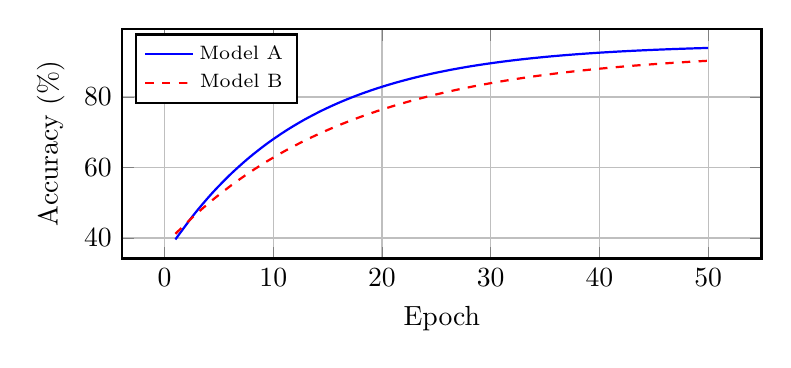
\begin{tikzpicture}
				\begin{axis}[
					width=0.8\textwidth,
					height=45mm,
				 xlabel={Epoch},
				 ylabel={Accuracy (\%)},
				 legend style={font=\scriptsize, at={(0.02,0.98)}, anchor=north west},
				 grid=major,
				 thick,
				]
					\addplot[blue, thick, smooth, domain=1:50, samples=30]
						{95 - 60*exp(-0.08*x)};
					\addlegendentry{Model A}
					\addplot[red, thick, dashed, smooth, domain=1:50, samples=30]
						{93 - 55*exp(-0.06*x)};
					\addlegendentry{Model B}
				\end{axis}
			\end{tikzpicture}
		\end{posterblocknotitle}
	\end{posterblock}

	\columnbreak

	\begin{posterblock}[Architecture Overview]
		\begin{posterblocknotitle}
			\centering
			\begin{tikzpicture}[
				box/.style={draw, thick, rounded corners, minimum height=8mm,
					     minimum width=18mm, fill=blue!10, font=\scriptsize},
				arr/.style={->, thick, >=stealth},
				node distance=8mm,
			]
				\node[box] (user) {User};
				\node[box, below=of user] (api) {API Layer};
				\node[box, below left=of api] (db) {Database};
				\node[box, below right=of api] (cache) {Cache};
				\node[box, below right=of db] (storage) {Storage};
				\draw[arr] (user) -- (api);
				\draw[arr] (api) -- (db);
				\draw[arr] (api) -- (cache);
				\draw[arr] (db) -- (storage);
				\draw[arr] (cache) -- (storage);
			\end{tikzpicture}
		\end{posterblocknotitle}
	\end{posterblock}

	\begin{posterblock}[References]
		\small
		\begin{enumerate}
			\item KOMA-Script Documentation, \texttt{ctan.org/pkg/koma-script}
			\item LaTeX Project Team, \textit{The \LaTeX{} Companion}, 2023
			\item OmniLaTeX Repository, \texttt{github.com/WyattAu/OmniLaTeX-template}
		\end{enumerate}
	\end{posterblock}

\end{multicols}

\end{document}
